\section{Description of Dataset, Task and Evaluation}
\label{sec:3}

In this section we introduce the target dataset, the structure of articles and the relationship between articles which is regarded as a graph, called corpus-graph. Then, we bring forward the task of our work that a framework or a recommendation system is designed to discover related articles automatically instead of accomplishing the job manually. The final goals is to make the break-even point between the precision of predicting and the operating performance. In the end of the section, we discuss which evaluation methods are chosen and the reason thereof. 

\subsection{Description of Dataset}
\label{sec:3.1}

Our task concentrates on the corpus \textbf{ZEIT} ONLINE. ``DIE ZEIT'' (eng. ``the time'') is a German national weekly newspaper and ``ZEIT ONLINE''\footnote{ZEIT ONLINE: http://www.zeit.de/index} is the corresponding online representation. More than 300,000 articles, which are released between 1946 and 2014 and marked into 20 different categories, are collected in the corpus. Basically, one or two articles are indicated as recommended reading for each article. In the past, normally, this kind of assignments is completed by editors manually. The motivation of this research is to find an automatic or semiautomatic alternative approach to accomplish the job. Foremost, the elementary information and statistic are useful for a better understanding of the corpus. 

\subsubsection{Meta-data and Structure}
\label{sec:3structure}

The record of each article consists of a structure of meta-data, which describe the elementary information of the article. The structure is introduced briefly in this section. Then a typical example is depicted in figure~\ref{fig:article_structure}.



\begin{description}
    \item[URL] the hyperlink as the entry to access the article.

    \item[Title] a descriptive heading or caption, in which the article is summarized.
    \item[Supertitle] a label of the article, which indicates a particular theme under the category.
    \item[Summary] a couple of sentences where is used for arousing the interest of reader and which are the explanation of the background or the summarization of the article. 
    \item[Author] the writer of the article.
    \item[Release date] the timestamp of publishing the article..
    \item[Category] the category which the article belongs to..

    \item[Content] the main body of the article.
    
    \item[Keywords] a couple of nouns or phrases which are significant for the article and can be used for retrieval. Normally, the vocabulary of all possible keywords is maintained manually. 
    
    \begin{figure}[!htb]
    \centering
    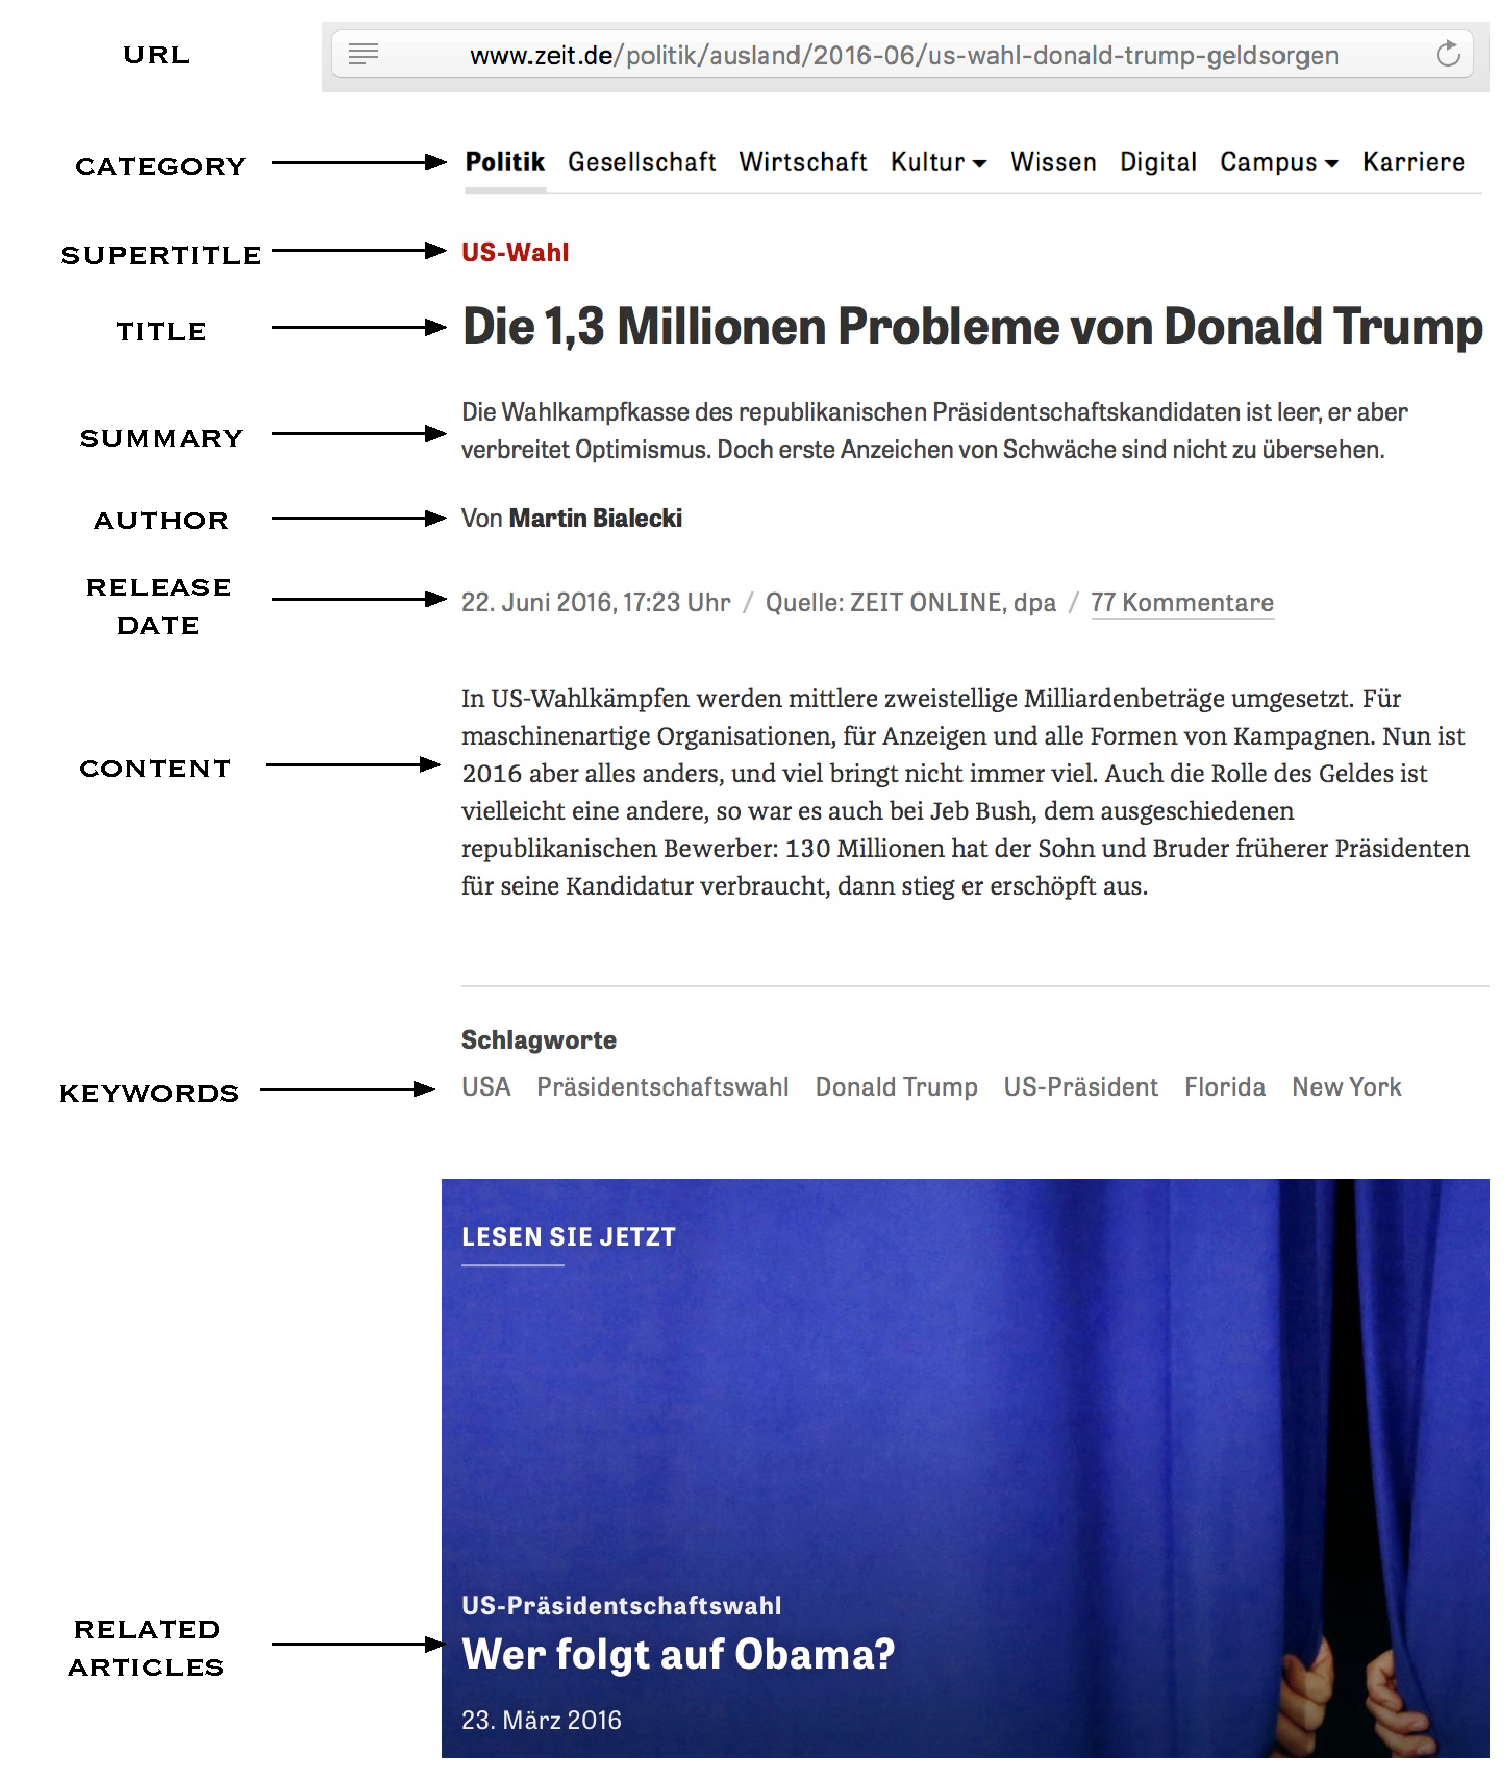
\includegraphics[width=1\textwidth]{fig/article.pdf}
    \caption{a typical example of the structure and meta-data of articles}
    \label{fig:article_structure}
    \end{figure}
    
    \item[Related articles] the recommendation for extended reading according to the current article. The related articles may have the same topic, similar background, or causal relationship to the current article.

        
\end{description}

\subsubsection{Relatedness and Corpus-Graph}

As introduced in the previous section, each article has one or two recommended articles. From the viewpoint of graph theory, the corpus is treated as a undirected graph, in which articles are regarded as vertices and the relationship of recommendation are as edges between the target article and recommended articles. Formally, two articles can be labeled as ``related''-by-$h$ to each other, if a path between them exists in the path and the length thereof is shorted than the pre-defined value $h$ (by default: 3). For instance represented in figure \ref{fig:relatedness}, article $A$ is related to article $B, C, D, E, F, F, G$, and unrelated to  article $H$ (too far from the target), $I, J, K$ (unreachable from the target). 
 
\begin{figure}[!htb]
    \centering
    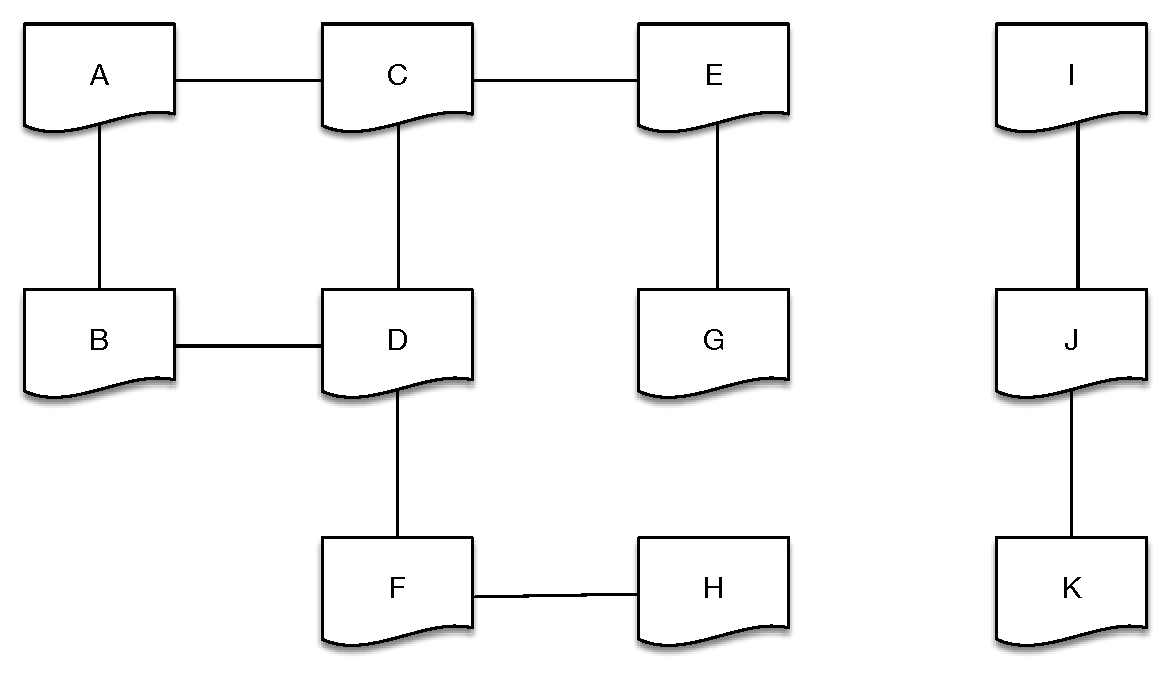
\includegraphics[width=0.75\textwidth]{fig/relatedness.pdf}
    \caption{a schematic graph of articles and relationship of relatedness}
    \label{fig:relatedness}
\end{figure}


\subsection{Description of Task}
\label{sec:3.2}

In the past, the relationship of relatedness are labeled typically by the author. However, this way has some disadvantages. On the one hand, the job need more human costs. On the other hand, the selection of candidates is limited by the work capacity and knowledge of the author, and these level is not stable. So it is necessary to exploit an automatic framework to discover related articles. The input of the framework is a article represented in a structure described in section~\ref{sec:3structure}, while the output is $k$ (in our case, $k=2$) articles which are marked as ``related'' normally with highest score or probability computed by the model. After determining the input and the expected output format, the main task is to train the model with the corpora of historical articles. The training methods are classified into unsupervised and supervised methods. The both kinds of methods are elaborated in section~\ref{sec:xxx}. In the scenario of reality, articles come in chronological order and the corpora which is as dataset of candidates has to be updated timely, because articles which are close to each other in time prefer to be more related than articles which are distant in time (see section \ref{sec:yyy}). Furthermore, it is also essential to update the model, in order to improve the precision, while operation of updating is costly and will lead to decrease the operating performance. Another task is, hence, to find an incremental method of updating and the trade-off between the effectiveness (precision) and efficiency (operating performance). The high-level depiction is drawn in figure~\ref{fig:highlevel}. 

\begin{figure}[!htb]
    \centering
    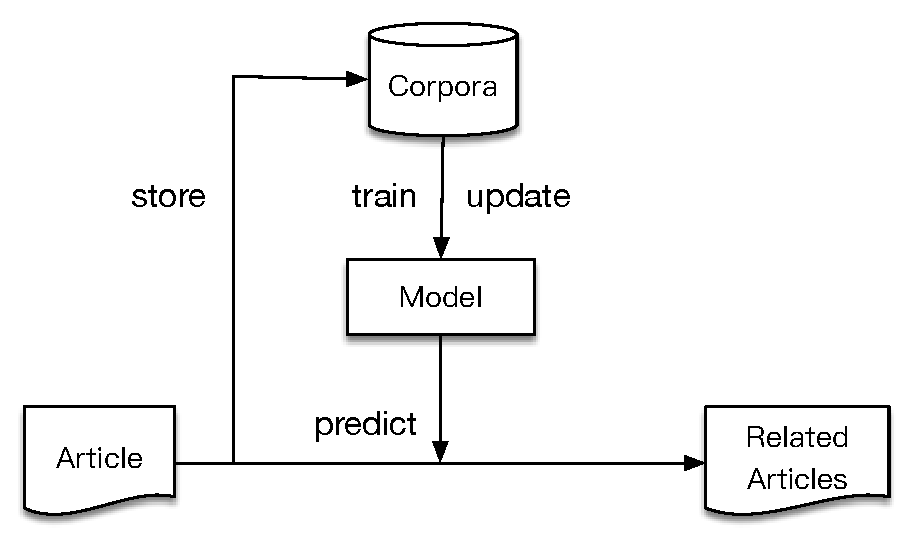
\includegraphics[width=0.6\textwidth]{fig/high-level.pdf}
    \caption{High-level depiction of the framework to discover related articles. }
    \label{fig:highlevel}
\end{figure}

\subsection{Evaluation Method}
\label{sec:3.3}

Effectiveness and efficiency are two main performance indicator. Effectiveness is about doing the right things. particularly in our case, it refers to whether the framework discovers related articles. Efficiency is about doing the things in optimal way, i.e., how much time and memory usage a series of operations to find related articles consumes. 

\subsubsection{Effectiveness}

The evaluation of effectiveness can be separated into two parts. One of them is to evaluate how well the final results and the other one is to indicate how well the entire ranking of candidates are computed by the framework given the target article. \textit{Precision@k@h} is used for the former and \textit{normalized Discounted Cumulative Gain} (\textit{nDCG}) is applied for the latter. 

\textit{Precision@k@h} is defined as the ratio of the number of the correct predictions to the number of predictions. Formally, given the corpora $D = \{d_1, d_2, \cdots, d_n\}$, a target set $T = \{t_1, t_2, \cdots, t_s\}$, the framework predicts $k$ related articles $P_i = \{d_{i_1}, \cdots, d_{i_k}\}$ for each article $i$ in $T$. Articles, which are at most $h$-hops apart from the target article, are regarded as the set $R_i^h$ of the true related articles of the article $i$ in $T$. 
\begin{equation}
    precision@k@h = \frac{\sum_{i=1}^s{|P_i \cap R_i^h|}}{k \cdot |T|}
\end{equation}

Unlike \textit{precision@k@h} which is applied to evaluate the final results of the framework, \textit{nDCG}, which is a measure of ranking quality in the field of information retrieval, focuses to evaluate the relatedness degree of the entire candidates. The framework makes a ranking of all $n$ candidates by the relatedness score or probability for a given target article $t$. Note that a article $d_i$ is placed at the position $i$ in the ranking. The relatedness degree is defined as $2^{-l}$ where $l$ is the distance between two articles in the corpus-graph.\footnote{$l=+\infty$ and the degree is $0$, if the articles are unreachable to each other.} We denote the degree between the target $t$ and a candidate $d_i$ by $ref_{d_i}^t$.

The formula to compute \textit{nDCG} of a target article $t$ is as followed. 

\begin{align}
   & nDCG_t = \frac{DCG_t}{IDCG_t} = (\sum_{i=1}^n\frac{ref_{d_i}^t-1}{log_2(i+1)})/(\sum_{i=1}^n\frac{ref_{d_i}^t-1}{log_2(r_{d_i}+1)})
\end{align}

Where $r_{d_i}$ is the position of $d_i$ of the ideal ranking which is generated by ordering by the relatedness degree. The \textit{nDCG} of the target set is $nDCG = \sum_{t \in T}nDCG_t$/s.

\subsubsection{Efficiency}

The newspaper is quite time-sensitive, so that it is significant that all tasks inclusive of discovery related articles should be completed as soon as possible. The time and memory usage of building model, predicting and updating model should be evaluated respectively. We focus mainly on the divergence between different methods in order to compare their relative merits, whereas the concrete value of time cost and memory usage depends on the performance of hardware and hence we discuss just whether the cost is in a reasonable range. For instance, the operation of predicting should be finshed in one minute maximal and it is reasonable and tolerable that building model is completed in one day or even a couple days. 